\documentclass[tikz,border=3pt]{standalone}
\usepackage[T1]{fontenc}
\usepackage{mathptmx}
\usetikzlibrary{arrows.meta,calc,decorations.pathreplacing}
\begin{document}
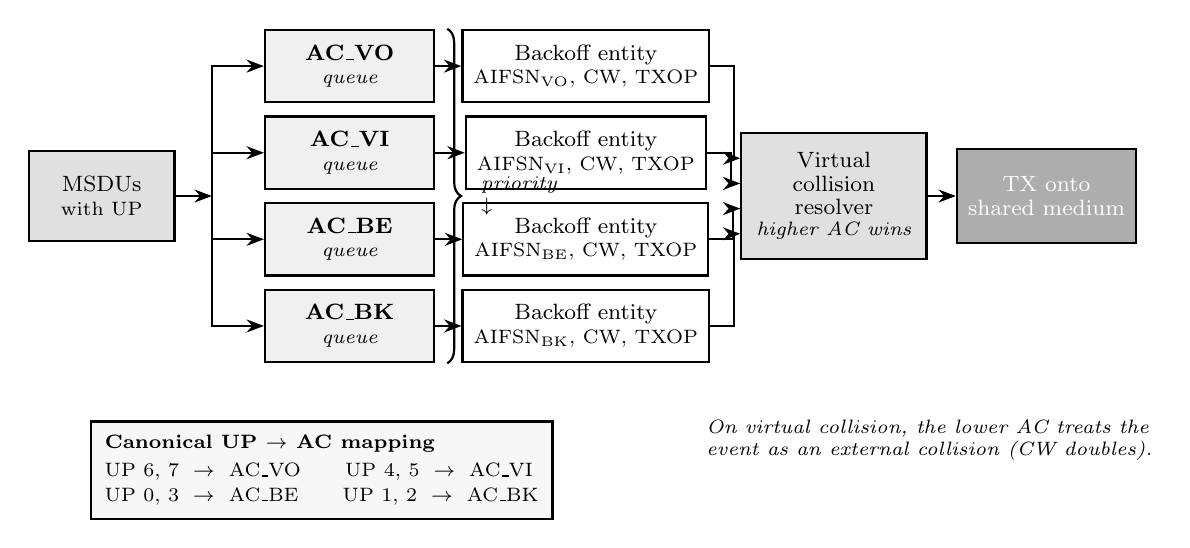
\begin{tikzpicture}[
  font=\footnotesize,
  >=Stealth,
  thick,
  box/.style={draw, thick, align=center, inner sep=4pt},
  queue/.style={box, minimum width=2.15cm, minimum height=0.92cm, fill=black!6},
  backoff/.style={box, minimum width=2.70cm, minimum height=0.92cm, fill=white},
  stage/.style={box, fill=black!12},
  sink/.style={box, minimum width=2.20cm, minimum height=1.20cm, fill=black!32, text=white},
  mapbox/.style={draw, thick, align=left, inner sep=5pt, fill=black!3, font=\scriptsize},
  lbl/.style={font=\scriptsize\itshape},
  arr/.style={-{Stealth[length=2.2mm]}, thick},
]
  % Incoming
  \node[stage, minimum width=1.85cm, minimum height=1.15cm] (msdu) at (0.0,2.40)
    {MSDUs\\[-1pt]{\scriptsize with UP}};

  % AC queues (VO highest)
  \node[queue] (qVO) at (3.15,4.05) {\textbf{AC\_VO}\\[-1pt]{\scriptsize\itshape queue}};
  \node[queue] (qVI) at (3.15,2.95) {\textbf{AC\_VI}\\[-1pt]{\scriptsize\itshape queue}};
  \node[queue] (qBE) at (3.15,1.85) {\textbf{AC\_BE}\\[-1pt]{\scriptsize\itshape queue}};
  \node[queue] (qBK) at (3.15,0.75) {\textbf{AC\_BK}\\[-1pt]{\scriptsize\itshape queue}};

  % Backoff entities
  \node[backoff] (boVO) at (6.15,4.05)
    {Backoff entity\\[-1pt]{\scriptsize AIFSN$_{\mathrm{VO}}$, CW, TXOP}};
  \node[backoff] (boVI) at (6.15,2.95)
    {Backoff entity\\[-1pt]{\scriptsize AIFSN$_{\mathrm{VI}}$, CW, TXOP}};
  \node[backoff] (boBE) at (6.15,1.85)
    {Backoff entity\\[-1pt]{\scriptsize AIFSN$_{\mathrm{BE}}$, CW, TXOP}};
  \node[backoff] (boBK) at (6.15,0.75)
    {Backoff entity\\[-1pt]{\scriptsize AIFSN$_{\mathrm{BK}}$, CW, TXOP}};

  % Fan-out MSDU → queues
  \coordinate (hub) at (1.40,2.40);
  \draw[arr] (msdu.east) -- (hub);
  \draw[arr] (hub) |- (qVO.west);
  \draw[arr] (hub) |- (qVI.west);
  \draw[arr] (hub) |- (qBE.west);
  \draw[arr] (hub) |- (qBK.west);

  \draw[arr] (qVO) -- (boVO);
  \draw[arr] (qVI) -- (boVI);
  \draw[arr] (qBE) -- (boBE);
  \draw[arr] (qBK) -- (boBK);

  % Virtual collision resolver
  \node[stage, minimum width=2.35cm, minimum height=1.60cm] (vcr) at (9.30,2.40)
    {Virtual\\[-1pt]collision\\[-1pt]resolver\\[-2pt]
     {\scriptsize\itshape higher AC wins}};

  \draw[arr] (boVO.east) -- ++(0.30,0) |- ($(vcr.west)+(0,0.48)$);
  \draw[arr] (boVI.east) -- ++(0.30,0) |- ($(vcr.west)+(0,0.16)$);
  \draw[arr] (boBE.east) -- ++(0.30,0) |- ($(vcr.west)+(0,-0.16)$);
  \draw[arr] (boBK.east) -- ++(0.30,0) |- ($(vcr.west)+(0,-0.48)$);

  % Shared medium
  \node[sink] (tx) at (12.00,2.40) {TX onto\\[-1pt]shared medium};
  \draw[arr] (vcr) -- (tx);

  % Brace: priority order
  \draw[decorate, decoration={brace, amplitude=5pt, raise=2pt}, thick]
    ($(qVO.north east)+(0.08,0)$) -- ($(qBK.south east)+(0.08,0)$);
  \node[lbl, anchor=west, align=left] at ($(qVO.east)!0.5!(qBK.east)+(0.45,0)$)
    {priority\\$\downarrow$};

  % Mapping panel
  \node[mapbox, anchor=north west] at (-0.15,-0.45) {%
    \textbf{Canonical UP $\rightarrow$ AC mapping}\\[2pt]
    UP 6, 7 $\;\rightarrow\;$ AC\_VO\qquad
    UP 4, 5 $\;\rightarrow\;$ AC\_VI\\[1pt]
    UP 0, 3 $\;\rightarrow\;$ AC\_BE\qquad
    UP 1, 2 $\;\rightarrow\;$ AC\_BK};

  \node[lbl, anchor=west, align=left] at (7.55,-0.70) {%
    On virtual collision, the lower AC treats the\\
    event as an external collision (CW doubles).};
\end{tikzpicture}
\end{document}
